%%%%%%%%%%%%%%%%%%%%%%%%%%%%%%%%%%%%

\section{$t$分布を用いた1標本平均の推測}

%%%%%%%%%%%%%%%%%%%%%%%%%%%%%%%%%%%%

\begin{frame}
\frametitle{13日の金曜日}

\dq{1990年から1992年にかけて、英国の研究者たちが13日の金曜日とその前週の金曜日（6日）の交通量、事故件数、入院件数に関するデータを収集した。以下は交通量に関するデータの抜粋である。場所1と場所2の交通量は独立であると仮定できる。}

{\scriptsize
\texttt{
\begin{center}
\begin{tabular}{rllrrrl}
  \hline
 & 種別 & 日付 & 6日 & 13日 & 差 & 場所  \\
  \hline
1 & 交通量 & 1990年7月 & 139246 & 138548 & 698 & 場所1 \\
  \rowcolor[gray]{.9}
  2 & 交通量 & 1990年7月 & 134012 & 132908 & 1104 & 場所2 \\
  3 & 交通量 & 1991年9月 & 137055 & 136018 & 1037 & 場所1 \\
  \rowcolor[gray]{.9}
  4 & 交通量 & 1991年9月 & 133732 & 131843 & 1889 & 場所2 \\
  5 & 交通量 & 1991年12月 & 123552 & 121641 & 1911 & 場所1 \\
  \rowcolor[gray]{.9}
  6 & 交通量 & 1991年12月 & 121139 & 118723 & 2416 & 場所2 \\
  7 & 交通量 & 1992年3月 & 128293 & 125532 & 2761 & 場所1 \\
  \rowcolor[gray]{.9}
  8 & 交通量 & 1992年3月 & 124631 & 120249 & 4382 & 場所2 \\
  9 & 交通量 & 1992年11月 & 124609 & 122770 & 1839 & 場所1 \\
  \rowcolor[gray]{.9}
  10 & 交通量 & 1992年11月 & 117584 & 117263 & 321 & 場所2 \\
   \hline
\end{tabular}
\end{center}
}}

\vfill

\rule{2.5cm}{0.25pt} \\
{\tiny Scanlon, T.J., Luben, R.N., Scanlon, F.L., Singleton, N. (1993), ``Is Friday the 13th Bad For Your Health?," BMJ, 307, 1584-1586.}

\end{frame}

%%%%%%%%%%%%%%%%%%%%%%%%%%%%%%%%%%%

\begin{frame}
\frametitle{13日の金曜日}

\begin{itemize}

\item 13日の金曜日と6日の金曜日で人々の行動が異なるかを調べたい。

\item 一つのアプローチは、この2つの日の交通量を比較することである。

\item $H_0:$ 6日と13日の金曜日の平均交通量は等しい。\\
$H_A:$ 6日と13日の金曜日の平均交通量は異なる。

\end{itemize}

$\:$ \\

\dq{データセットの各ケースは、同じ場所・同じ月・同じ年に記録された交通量を表している：6日の金曜日のカウントと13日の金曜日のカウントである。この2つのカウントは独立か？}

\soln{いいえ}

\end{frame}

%%%%%%%%%%%%%%%%%%%%%%%%%%%%%%%%%%%

\begin{frame}
\frametitle{仮説}

\pq{6日と13日の金曜日の平均交通量の差を検定するための仮説はどれか？}

\begin{enumerate}[(a)]
\item  \mathhl{H_0:} $\mu_{6th} = \mu_{13th}$ \\
\mathhl{H_A:} $\mu_{6th} \ne \mu_{13th}$
\item  \mathhl{H_0:} $p_{6th} = p_{13th}$ \\
\mathhl{H_A:} $p_{6th} \ne p_{13th}$
\solnMult{ \mathhl{H_0:} $\mu_{diff} = 0$ \\
\mathhl{H_A:} $\mu_{diff} \ne 0$ }
\item  \mathhl{H_0:} $\bar{x}_{diff} = 0$ \\
\mathhl{H_A:} $\bar{x}_{diff} = 0$
\end{enumerate}

\end{frame}

%%%%%%%%%%%%%%%%%%%%%%%%%%%%%%%%%%%

\begin{frame}
\frametitle{条件の確認}

\begin{itemize}

\item \hl{独立性：} ケース（行）は独立であると仮定する。

\item \hl{標本サイズ／歪み：} $\:$ \\

\twocol{0.75}{0.35}
{
{\tiny
\begin{itemize}

\item 標本分布は極端に歪んでいるようには見えないが、標本サイズが非常に小さいため判断が難しい。母集団分布が歪んでいるかどうかを考える必要がある――おそらく平均より交通量が少ない日と多い日は同程度に起こりうるため、歪んではいないだろう。

\item $\sigma$は未知であり、$n$が小さすぎるため$s$が$\sigma$の信頼できる推定値とは言えない。
\end{itemize}
}
}
{
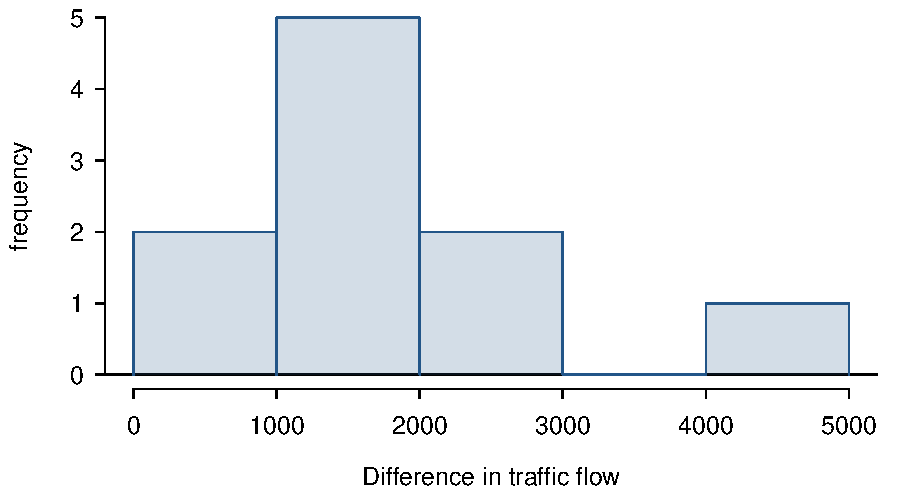
\includegraphics[width=\textwidth]{7-1_one_t/figures/friday/trafficHist}
}

\end{itemize}

$\:$ \\

\dq{では、標本サイズが小さい場合はどうすればよいか？}

\end{frame}

%%%%%%%%%%%%%%%%%%%%%%%%%%%%%%%%%%%

\begin{frame}
\frametitle{復習：大標本の役割}

観測値が独立であり、母集団分布が極端に歪んでいない限り、大標本によって次のことが保証される：

\begin{itemize}

\item 平均の標本分布がほぼ正規分布になる

\item 標準誤差の推定値$\frac{s}{\sqrt{n}}$が信頼できる

\end{itemize}

\end{frame}

%%%%%%%%%%%%%%%%%%%%%%%%%%%%%%%%%%%

\subsection{正規性の条件}

%%%%%%%%%%%%%%%%%%%%%%%%%%%%%%%%%%%

\begin{frame}
\frametitle{正規性の条件}

\begin{itemize}

\item 中心極限定理（CLT）によれば、母集団分布がほぼ正規であれば、\orange{いかなる}標本サイズでも標本分布はほぼ正規になる。

\item これは有用な特別なケースだが、小標本では正規性の確認が本質的に難しい。

\item 小標本における正規性の条件を確認する際は注意が必要である。データを調べるだけでなく、データの出所についても考えることが重要である。
\begin{itemize}
\item 例えば、この分布は対称であると期待できるか、また外れ値はまれであると確信できるか、という点を問うべきである。
\end{itemize}

\end{itemize}

\end{frame}

%%%%%%%%%%%%%%%%%%%%%%%%%%%%%%%%%%%

\subsection{$t$分布の紹介}

%%%%%%%%%%%%%%%%%%%%%%%%%%%%%%%%%%%

\begin{frame}
\frametitle{$t$分布}

\begin{itemize}

\item 母集団の標準偏差が未知の場合（ほぼ常にそうであるが）、標準誤差の推定の不確実性は\hl{$t$分布}という新しい分布を使用することで対処される。

\item この分布もベル形状をしているが、裾が正規分布より\hl{厚い}。

\item したがって、正規分布と比べて、平均から2SDを超える位置に観測値が落ちる可能性が高い。

\item 裾が厚いことは、標準誤差の推定が信頼性に欠ける場合（$n$が小さい場合）の問題を解決するのに役立つ。

\end{itemize}

\begin{center}
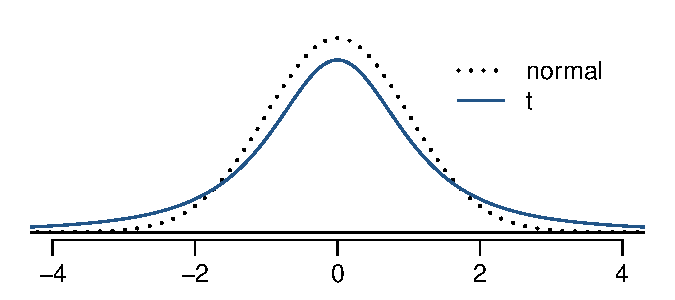
\includegraphics[width=0.5\textwidth]{7-1_one_t/figures/tDistCompareToNormalDist/tDistCompareToNormalDist}
\end{center}

\end{frame}

%%%%%%%%%%%%%%%%%%%%%%%%%%%%%%%%%%%

\begin{frame}
\frametitle{$t$分布（続き）}

\begin{itemize}

\item 標準正規（$z$）分布と同様に、常に0を中心とする。

\item パラメータは1つ：\hl{自由度}（\mathhl{df}）。

\end{itemize}

\begin{center}
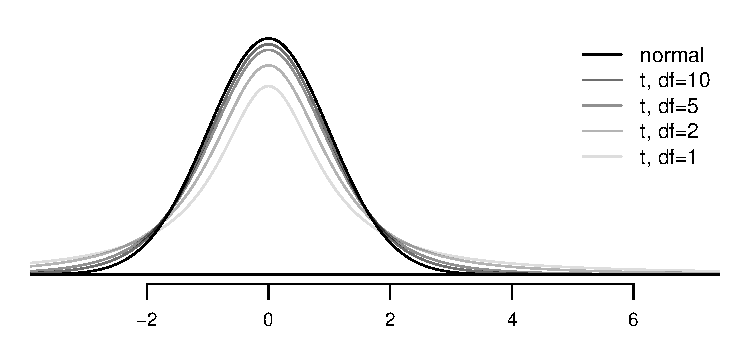
\includegraphics[width=0.8\textwidth]{7-1_one_t/figures/tDistConvergeToNormalDist/tDistConvergeToNormalDist}
\end{center}

\dq{$df$が増加すると$t$分布の形はどうなるか？}

\soln{正規分布に近づく。}

\end{frame}

%%%%%%%%%%%%%%%%%%%%%%%%%%%%%%%%%%%

\subsection{$t$分布を用いた仮説の検定}

%%%%%%%%%%%%%%%%%%%%%%%%%%%%%%%%%%%

\begin{frame}
\frametitle{13日の金曜日に戻ろう}

\vspace{-1cm}

{\footnotesize
\texttt{
\begin{center}
\begin{tabular}{rllrr || r || l}
  \hline
 & 種別 & 日付 & 6日 & 13日 & 差 & 場所  \\
  \hline
1 & 交通量 & 1990年7月 & 139246 & 138548 & 698 & 場所1 \\
  \rowcolor[gray]{.9}
  2 & 交通量 & 1990年7月 & 134012 & 132908 & 1104 & 場所2 \\
  3 & 交通量 & 1991年9月 & 137055 & 136018 & 1037 & 場所1 \\
  \rowcolor[gray]{.9}
  4 & 交通量 & 1991年9月 & 133732 & 131843 & 1889 & 場所2 \\
  5 & 交通量 & 1991年12月 & 123552 & 121641 & 1911 & 場所1 \\
  \rowcolor[gray]{.9}
  6 & 交通量 & 1991年12月 & 121139 & 118723 & 2416 & 場所2 \\
  7 & 交通量 & 1992年3月 & 128293 & 125532 & 2761 & 場所1 \\
  \rowcolor[gray]{.9}
  8 & 交通量 & 1992年3月 & 124631 & 120249 & 4382 & 場所2 \\
  9 & 交通量 & 1992年11月 & 124609 & 122770 & 1839 & 場所1 \\
  \rowcolor[gray]{.9}
  10 & 交通量 & 1992年11月 & 117584 & 117263 & 321 & 場所2 \\
   \hline
\end{tabular}
\end{center}
}}

\begin{align*}
\hspace{6cm} &\orange{$\bar{x}_{diff} = 1836$} \\
& \orange{$s_{diff} = 1176$} \\
& \orange{$n = 10$}
\end{align*}

\end{frame}

%%%%%%%%%%%%%%%%%%%%%%%%%%%%%%%%%%%

\begin{frame}
\frametitle{検定統計量の計算}

\formula{小標本平均の推測における検定統計量}
{小標本（$n < 30$）の平均に関する推測の検定統計量は、$df = n - 1$の$T$統計量である。
\[ T_{df} = \frac{\text{点推定量} - \text{帰無値}}{SE} \]}

\vspace{-0.5cm}

\hl{この文脈では…}
\begin{eqnarray*}
\text{点推定量} &=& \bar{x}_{diff} = 1836 \\
SE &=& \frac{s_{diff}}{\sqrt{n}} = \frac{1176}{\sqrt{10}} = 372 \\
T &=& \frac{1836 - 0}{372} = 4.94 \\
df &=& 10 - 1 = 9
\end{eqnarray*}

\vspace{-0.25cm}

\Note{帰無仮説で$\mu_{diff} = 0$と設定したため、帰無値は0である。}

\end{frame}

%%%%%%%%%%%%%%%%%%%%%%%%%%%%%%%%%%%

\begin{frame}[fragile]
\frametitle{p値の計算}

\begin{itemize}

\item p値は、再び$t$分布の裾の面積として計算される。

\item Rを使う場合：
\begin{verbatim}
> 2 * pt(4.94, df = 9, lower.tail = FALSE)

[1] 0.0008022394
\end{verbatim}

\item ウェブアプリを使う場合：

\href{https://gallery.shinyapps.io/dist_calc/}{\textcolor{oiB}{https://gallery.shinyapps.io/dist\_calc/}}

\item これらが利用できない場合は、$t$表を使うことができる。

\end{itemize}

\end{frame}

%%%%%%%%%%%%%%%%%%%%%%%%%%%%%%%%%%%


\begin{frame}
\frametitle{検定の結論}

\dq{この仮説検定の結論は何か？}

p値が非常に小さいため、データは6日と13日の金曜日の交通量に差があることを示す強い証拠を提供していると結論付ける。

\end{frame}

%%%%%%%%%%%%%%%%%%%%%%%%%%%%%%%%%%%%

\subsection{$t$分布を用いた信頼区間の構築}

%%%%%%%%%%%%%%%%%%%%%%%%%%%%%%%%%%%

\begin{frame}
\frametitle{差はどれくらいか？}

\begin{itemize}

\item 6日と13日の金曜日の交通量に差があると結論付けた。

\item しかし、その差が具体的にどれくらいかを知ることがより興味深い。

\item 信頼区間を使ってこの差を推定することができる。

\end{itemize}

\end{frame}

%%%%%%%%%%%%%%%%%%%%%%%%%%%%%%%%%%%

\begin{frame}
\frametitle{小標本平均の信頼区間}

\begin{itemize}

\item 信頼区間は常に次の形をとる：
\[ \text{点推定量} \pm {ME} \]

\item MEは常に、臨界値と標準誤差の積として計算される。

\item 小標本平均は$z$分布ではなく$t$分布に従うため、臨界値は$t^\star$（$z^\star$ではなく）となる：
\[ \text{点推定量} \pm t^{\star} \times SE \]

\end{itemize}

\end{frame}

%%%%%%%%%%%%%%%%%%%%%%%%%%%%%%%%%%%

\begin{frame}[fragile]
\frametitle{臨界値$t^\star$の計算}


Rを使う場合：
\begin{verbatim}

> qt(p = 0.975, df = 9)

[1] 2.262157

\end{verbatim}

\end{frame}

%%%%%%%%%%%%%%%%%%%%%%%%%%%%%%%%%%%

\begin{frame}
\frametitle{小標本平均の信頼区間の構築}

\pq{6日と13日の金曜日の交通量の差に対する95\%信頼区間の正しい計算はどれか？}
\[ \bar{x}_{diff} = 1836 \qquad s_{diff} = 1176 \qquad n = 10 \qquad SE = 372 \]

\twocol{0.35}{0.65}
{
\begin{enumerate}[(a)]

\item $1836 \pm 1.96 \times 372$

\solnMult{ $1836 \pm 2.26 \times 372$}

\item $1836 \pm -2.26 \times 372$

\item $1836 \pm 2.26 \times 1176$

\end{enumerate}
}
{
\only<2->{\orange{$\rightarrow$ (995, 2677)}}
\vspace{0.25cm}
}

\end{frame}

%%%%%%%%%%%%%%%%%%%%%%%%%%%%%%%%%%%

\begin{frame}
\frametitle{信頼区間の解釈}

\pq{先ほど計算した信頼区間の\orange{最も適切な}解釈はどれか？
\[ \mu_{diff: 6th - 13th} = (995, 2677) \]
}

95\%の確率で…

\begin{enumerate}[(a)]

\item 6日と13日の金曜日の平均交通量の差は995台から2,677台の間にある。

\item 6日の金曜日の方が13日の金曜日より平均して995台から2,677台少ない車が走っている。

\item 6日の金曜日の方が13日の金曜日より平均して995台少ないから2,677台多い車が走っている。

\solnMult{ 13日の金曜日の方が6日の金曜日より平均して995台から2,677台少ない車が走っている。}

\end{enumerate}

\end{frame}

%%%%%%%%%%%%%%%%%%%%%%%%%%%%%%%%%%%

\subsection{まとめ}

%%%%%%%%%%%%%%%%%%%%%%%%%%%%%%%%%%%

\begin{frame}
\frametitle{まとめ}

\dq{仮説検定の結論は信頼区間の結果と一致しているか？}

$\:$ \\

\soln{はい、仮説検定で有意な差が見られ、信頼区間は帰無値0を含んでいない。}

$\:$ \\

\dq{この研究の結果は、人々が13日の金曜日を不吉な日だと信じていることを示唆しているか？}

$\:$ \\

\soln{いいえ、これは観察研究である。この2日間の道路上の車の台数に有意な差があることを観察したに過ぎない。人々の信念を検定したわけではない。}

\end{frame}

%%%%%%%%%%%%%%%%%%%%%%%%%%%%%%%%%%%

\begin{frame}
\frametitle{まとめ：$t$分布を用いた推測}

\begin{itemize}

\item $\sigma$が未知の場合は、$SE = \frac{s}{\sqrt{n}}$として$t$分布を使用する。

\item 条件：
\begin{itemize}
\item 観測値の独立性（ランダム標本により確認、非復元抽出の場合は$n < $母集団の10\%）
\item 極端な歪みがない
\end{itemize}

\item 仮説検定：
\[ T_{df} = \frac{\text{点推定量} - \text{帰無値}}{SE}\text{，ただし }df = n - 1 \]

\item 信頼区間：$\text{点推定量} \pm t_{df}^\star \times SE$

\end{itemize}

\vspace{-0.25cm}

\Note{ここで使った例は対データの平均（従属グループ間の差）に関するものであった。観測値の差を取り、その差だけ（1標本）を分析に使用したため、1標本の場合と同じ手順となる。}

\end{frame}

%%%%%%%%%%%%%%%%%%%%%%%%%%%%%%%%%%%
